% LaTEX source code
% Last modified November 1st, 2005
% Steve Miller
% note that the percent sign comments out the rest of the line
% first, we set a document class. often use 12pt characters, though
% sometimes people do 11 or 10. you can do report or article, both similar
%\documentclass[12pt,letterpaper]{article}
\documentclass[12pt,reqno]{amsart}
\linespread{1}
\addtolength{\textwidth}{2cm} \addtolength{\hoffset}{-1cm}
\addtolength{\marginparwidth}{-1cm} \addtolength{\textheight}{2cm}
\addtolength{\voffset}{-1cm}
% below are some packages that are needed for certain symbols, graphics, colors.
% safest to just include these.
\usepackage{times}
\usepackage[T1]{fontenc}
\usepackage{mathrsfs}
\usepackage{latexsym}
\usepackage[dvips]{graphics}
\usepackage{epsfig}
\usepackage{hyperref, amsmath, amsthm, amsfonts, amscd, flafter,epsf}
\usepackage{amsmath,amsfonts,amsthm,amssymb,amscd}
\input amssym.def
\input amssym.tex
\usepackage{color}
\usepackage{enumerate}
\usepackage{hyperref}
\usepackage{url}
\usepackage{floatrow}
\usepackage{caption}
\usepackage{subcaption}
\usepackage{capt-of}
\usepackage{physics}
\newcommand{\todo}[1]{\textcolor{red}{\textbf{(#1)}}}

    %=======================================================

    %   THIS IS WHERE YOU PUT SHORTCUT DEFINITIONS

    %========================================================

% Note that we use a percent sign to comment out a line

% below are shortcut commands

%%%%%%%%%%%%%%%%%%%%%%%%%%%%%%%%%%%%%%%%%%%%%%%

% below are shortcuts for equation, eqnarray,

% itemize and enumerate environments

\newcommand\be{\begin{equation}}
\newcommand\ee{\end{equation}}
\newcommand\bea{\begin{eqnarray}}
\newcommand\eea{\end{eqnarray}}
\newcommand\bi{\begin{itemize}}
\newcommand\ei{\end{itemize}}
\newcommand\ben{\begin{enumerate}}
\newcommand\een{\end{enumerate}}
\newcommand{\ncr}[2]{\left({#1 \atop #2}\right)}
%%%%%%%%%%%%%%%%%%%%%%%%%%%%%%%%%%%%%%%%%%%%%%%%

% Theorem / Lemmas et cetera

\newtheorem{thm}{Theorem}[section]
\newtheorem{conj}[thm]{Conjecture}
\newtheorem{cor}[thm]{Corollary}
\newtheorem{lem}[thm]{Lemma}
\newtheorem{prop}[thm]{Proposition}
\newtheorem{exa}[thm]{Example}
\newtheorem{defi}[thm]{Definition}
\newtheorem{exe}[thm]{Exercise}
\newtheorem{rek}[thm]{Remark}
\newtheorem{que}[thm]{Question}
\newtheorem{prob}[thm]{Problem}
\newtheorem{cla}[thm]{Claim}
\newtheorem{defis}[thm]{Definitions}
\newtheorem{res}[thm]{Result}
\newtheorem{calc}[thm]{Calculation}
%%%%%%%%%%%%%%%%%%%%%%%%%%%%%%%%%%%%%%%%%

% shortcuts to environments

% this allows you to do textboldface: simply type \tbf{what you want in bold}

\newcommand{\tbf}[1]{\textbf{#1}}

%%%%%%%%%%%%%%%%%%%%%%%%%%%%%%%%%%%%%%%%%%%%%%%%%%

% shortcut to twocase and threecase definitions

\newcommand{\twocase}[5]{#1 \begin{cases} #2 & \text{#3}\\ #4
&\text{#5} \end{cases}   }
\newcommand{\threecase}[7]{#1 \begin{cases} #2 &
\text{#3}\\ #4 &\text{#5}\\ #6 &\text{#7} \end{cases}   }
%%%%%%%%%%%%%%%%%%%%%%%%%%%%%%%%%%%%%%%%%

%Blackboard Letters

\newcommand{\R}{\ensuremath{\mathbb{R}}}
\newcommand{\C}{\ensuremath{\mathbb{C}}}
\newcommand{\Z}{\ensuremath{\mathbb{Z}}}
\newcommand{\Q}{\mathbb{Q}}
\newcommand{\N}{\mathbb{N}}
\newcommand{\F}{\mathbb{F}}
\newcommand{\W}{\mathbb{W}}
\newcommand{\Qoft}{\mathbb{Q}(t)}  %use in linux
\newcommand{\soln}{\noindent \textbf{Solution:}\ }

%%%%%%%%%%%%%%%%%%%%%%%%%%%%%%%%%%%%%%%%%

% Finite Fields and Groups

\newcommand{\Fp}{ \F_p }
%%%%%%%%%%%%%%%%%%%%%%%%%%%%%%%%%%%%%%%%%

% Fractions

\newcommand{\foh}{\frac{1}{2}}  %onehalf
\newcommand{\fot}{\frac{1}{3}}
\newcommand{\fof}{\frac{1}{4}}

%%%%%%%%%%%%%%%%%%%%%%%%%%%%%%%%%%%%%%%%%

% Legendre Symbols

\newcommand{\js}[1]{ { \underline{#1} \choose p} }

%%%%%%%%%%%%%%%%%%%%%%%%%%%%%%%%%%%%%%%%%

% matrix shortcuts

\newcommand{\mattwo}[4]
{\left(\begin{array}{cc}
                        #1  & #2   \\
                        #3 &  #4
                          \end{array}\right) }
\newcommand{\matthree}[9]
{\left(\begin{array}{ccc}
                        #1  & #2 & #3  \\
                        #4 &  #5 & #6 \\
                        #7 &  #8 & #9
                          \end{array}\right) }
\newcommand{\dettwo}[4]
{\left|\begin{array}{cc}
                        #1  & #2   \\
                        #3 &  #4
                          \end{array}\right| }
\newcommand{\detthree}[9]
{\left|\begin{array}{ccc}
                        #1  & #2 & #3  \\
                        #4 &  #5 & #6 \\
                        #7 &  #8 & #9
                          \end{array}\right| }
%%%%%%%%%%%%%%%%%%%%%%%%%%%%%%%%%%%%%%%%%

% greek letter shortcuts

\newcommand{\ga}{\alpha}                  %gives you a greek alpha
\newcommand{\gb}{\beta}
\newcommand{\gep}{\epsilon}
%%%%%%%%%%%%%%%%%%%%%%%%%%%%%%%%%%%%%%%%%

% general functions

\newcommand{\notdiv}{\nmid}               % gives the not divide symbol
\newcommand{\burl}[1]{\textcolor{blue}{\url{#1}}}

%%%%%%%%%%%%%%%%%%%%%%%%%%%%%%%%%%%%%%%%%%%

% the following makes the numbering start with 1 in each section;

% if you want the equations numbered 1 to N (without caring about

% what section you are in, comment out the following line.

\numberwithin{equation}{section}

%\textwidth= 6in

%\evensidemargin=37pt

%\oddsidemargin=0pt

\begin{document}



\title{Machine Learning Results Log Summer 2018 (August - Present)}
\author{Kirk Swanson}
\email{swansonk1@uchicago.edu}
\address{Institute for Molecular Engineering, University of Chicago, 5640 S Ellis Ave, Chicago, IL 60637}
%\keywords{path integral molecular dynamics, path integral monte carlo, metropolis algorithm}
\date{\today}

\maketitle

\section{8/6/2018}
\begin{enumerate}
\item Going back to tutorial section about implementing an example GCN.  On Midway 2 gpu2, following the usual instructions.  
\item Briefly doing the PyTorch introduction: https://pytorch.org/tutorials/beginner/blitz/tensor\_tutorial.html
\end{enumerate}

\section{8/8/2018}
\begin{enumerate}
\item On https://github.com/rusty1s/pytorch\_geometric, looking at torch\_geometric/data/dataset.py.  We will go through this and understand line-by-line, because we want to create and load our own custom dataset.
\item "import collections".  From python documentation, collections "This module implements specialized container datatypes providing alternatives to Python's general purpose built-in containers, dict, list, set, and tuple.  Counter, for example, counts the number of examples of each class in a list.  "os.path".  From doc, "This module implements some useful functions on pathnames.  To read or write files see open(), and for accessing the filesystem see the os module."  
\item Now reading the Data Loading and Processing Tutorial on PyTorch: https://pytorch.org/tutorials/beginner/data\_loading\_tutorial.html.  "torch.utils.data.Dataset is an abstract class representing a dataset.  Your custom dataset should inherit Dataset and override the following methods: \_\_len\_\_ so that len(dataset) returns the size of the dataset, and \_\_getitem\_\_ to support the indexing such that dataset[i] can be used to get the ith sample."  Transforms can often be written using \_\_init\_\_ method as well as \_\_call\_\_ method.  
\end{enumerate}

\section{8/20/2018}
\begin{enumerate}
\item The following describes issues related to the inherent structure energy, $E_{IS}$, computed in liquid-cooled simulations used for my proposed research project, "Deep Learning for Glassy Physics."  The question of the origin of $E_{IS}$ values came up during a talk I was giving to Professors de Pablo, Galli, and Skinner on 8/19/2018, with Rovana present.  Professor Skinner asked what my computed $E_{IS}$ values represented, which are on the order of -4.0 (Lennard-Jones units) for a binary mixture of 4,320 particles interacting according to a Lennard-Jones force.  I suggested that these values represent the total energy of a minimized configuration, while he argued that they  represent the energy per particle of a configuration.  I was unable to resolve the issue on the spot and instead said that I would be happy to review the issue after the talk.  
\par In order to resolve the issue, and to explain why I was suggesting that these $E_{IS}$ values were total energy values, I first turned to the paper "Age and structure of a model vapour-deposited glass," by Reid et al.  My liquid-cooled simulation parameters and methdology are derived directly from this paper, not only because it provides clear instructions for performing this type of computation, but also because I wanted to ensure similarity between my data and that of Reid et al.  My machine learning project is attempting to answer questions raised in this paper, so it is important to produce simulations that have comparable characteristics.  For their 2D liquid-cooled systems, Reid et al. measure inherent structure energy values also to be on the order of -4.0.  The paper explains, "The inherent structure energy $E_{IS}$ of a configuration, used to quantify its stability, is the potential energy of a configuration brought to its local energy minimum."  This definition clearly suggests that $E_{IS}$ is a total energy value, and no where else in the paper is the energy defined to be a per atom or per particle quantity.  \par
The following shows the LAMMPS script that I used to compute inherent structure energy values from snapshots of a simulation:

\begin{figure}[H]
\centering
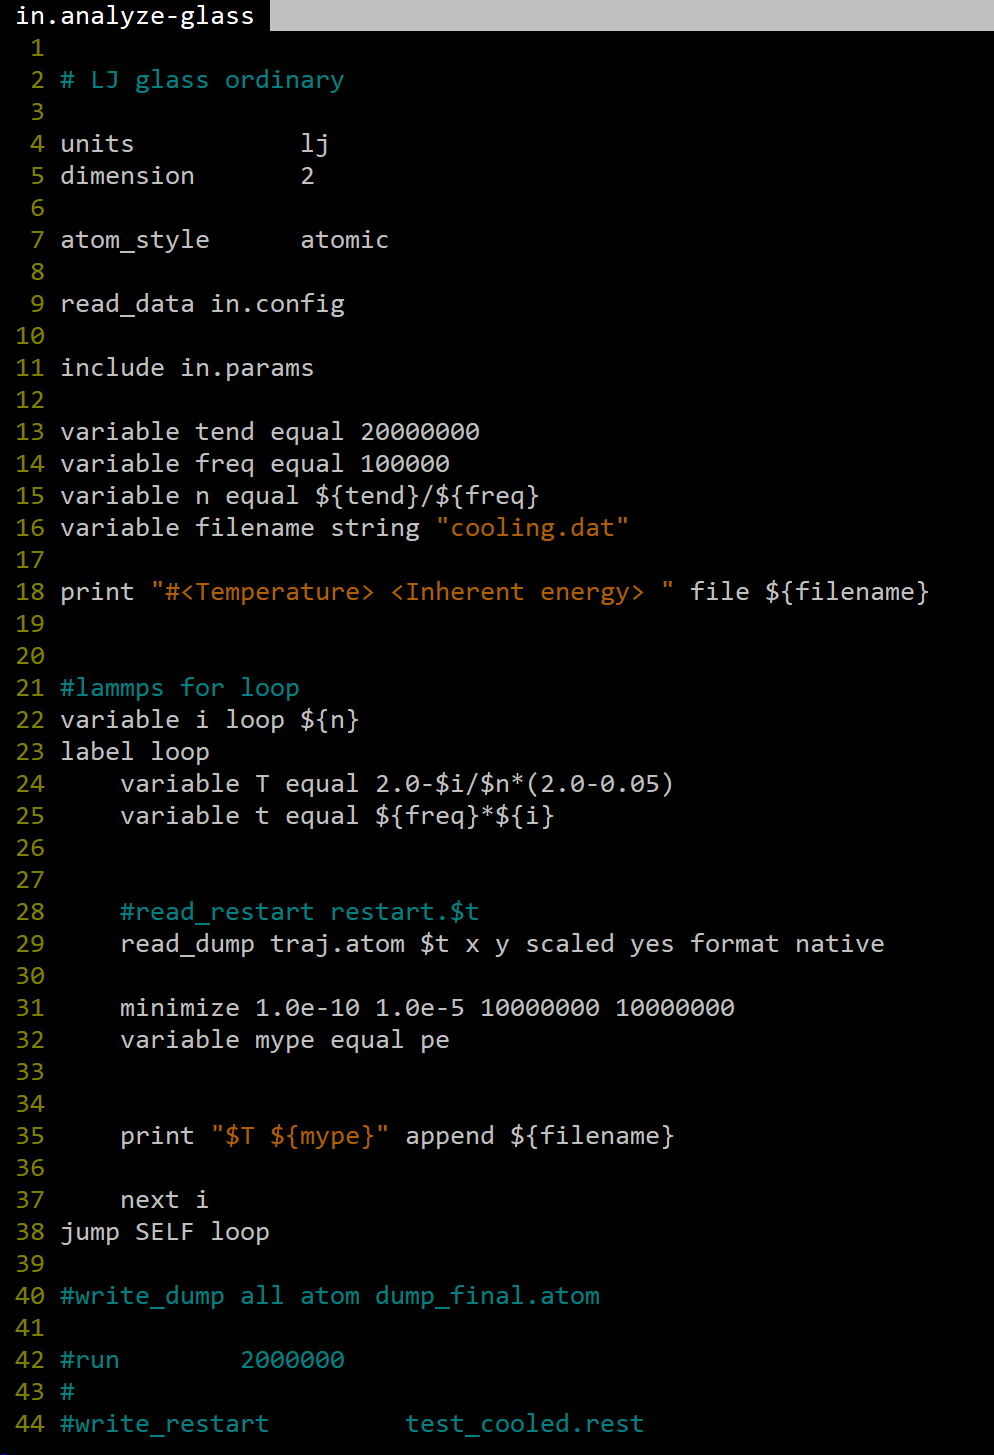
\includegraphics[scale=0.7]{energies}
\end{figure}

As shown above, a trajectory is read into the system, and then configurations every 100,000 steps are analyzed.  This analysis consists of three steps: perform an energy minimization (line 31), compute an energy (line 32), and print these values to an external file (line 35).  The energy computation on line 32, "variable mype equal pe" is responsible for computing the inherent structure energy.  The energy is taken from "pe", which is a variable pre-defined in LAMMPS and is described in official online documentation.  The documentation clearly defines "pe" as a total energy value.  The following is a screenshot from https://lammps.sandia.gov/doc/thermo\_style.html:

\begin{figure}[H]
\centering
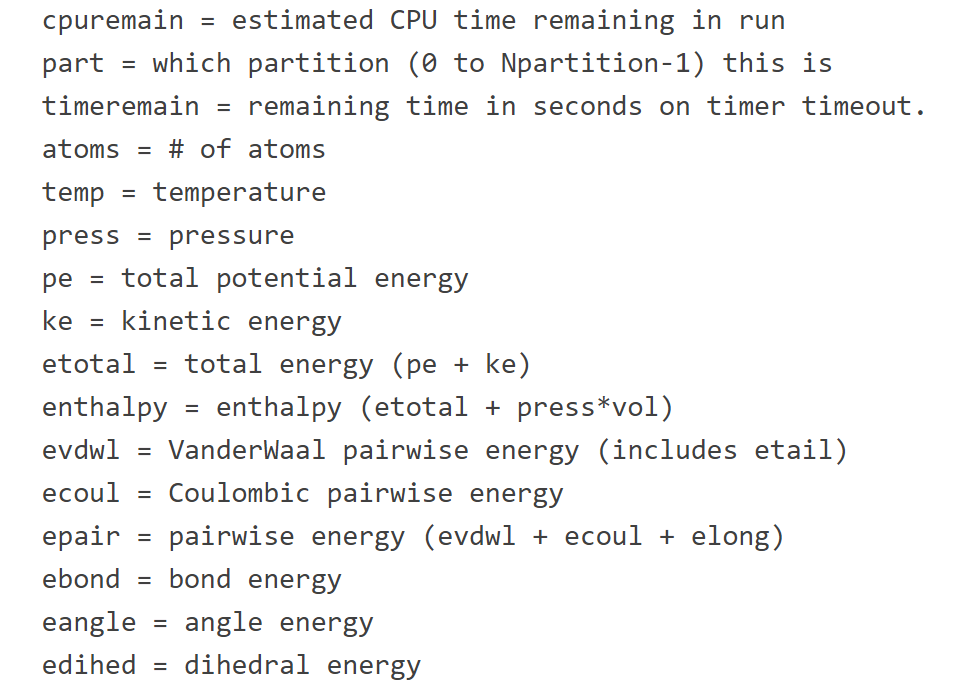
\includegraphics[scale=0.7]{lammps_pe}
\end{figure}



   


Reid et al.'s definition of inherent structure energy, as well as the energy computation command in my code, clearly explain why I suggested that my $E_{IS}$ values represent total potential energies rather than energies per atom.  I am currently working to definitively confirm the origins of computed $E_{IS}$ values to fully resolve this issue.      

\par Much more importantly,however, the distinction between the total energy of a configuration and the average energy per atom of a configuration does not impact my project or my results.  I am using this inherent structure energy value to compare the potential energy in different configurations that have the \textit{same number of particles}.  Therefore, making this comparison using total energy is equivalent to making the comparison using average energy per particle, and the type of comparison used has no impact on any  aspect of the project or the results that I have so far collected.    


\end{enumerate}

\section{9/11/2018}
\begin{enumerate}
\item First thing we are going to do is to create an actual dataset folder on midway.  Second thing will be to, step by step, build a custom dataset in PyTorch Geometric.  
\end{enumerate}



%%%%%%%%%%%%%%%%%%%%%%%%%%%%%%%%%%%%%%%%%%%%%%%%%%%%%%%%%%%%%%%%%%%%%%%%%%%%%%%%%%%%%%%%%%%%%%%%%%%%%%%%%%%%%%%%%%%%%%%%%%%%%%

\normalsize

%%%%%%%%%%%%%%%%%%%%%%%%%%%%%%%%%%%%%%%%%%%%%%%%%%%%%%%%%%%%%%%%%%%%%%%%%%%%%%%%%%%%%%%%%%%%%%%%%%%%%%%%%%%%%%%%%%%%%%%%%%%%%%


\end{document}